\documentclass[border=3pt,tikz]{standalone}
% Shared look for every TikZ figure in these notes.
% Included by each standalone figure file; also keeps the figures consistent
% with the colours used in the PDF and on the website.

\usepackage{tikz}
\usepackage{pgfplots}
\pgfplotsset{compat=1.18}
\usetikzlibrary{arrows.meta, decorations.markings, decorations.pathmorphing,
                patterns, calc, positioning}
\usepackage{amsmath}

% Series colours are the three validated categorical slots also used by the
% interactive widgets, so a path drawn in the printed notes and the same path on
% the website are the same colour. They clear the colour-vision-deficiency and
% contrast checks as a set; every path is direct-labelled as well, so colour is
% never the only thing carrying identity.
\definecolor{duPurple}{HTML}{68246D}
\definecolor{duBlue}{HTML}{2A78D6}
\definecolor{duRed}{HTML}{EB6834}
\definecolor{duGreen}{HTML}{1BAF7A}
\definecolor{duGrey}{HTML}{4D4D4D}

\tikzset{
  % heavier default lines and arrow tips, so diagrams stay clear when zoomed
  every picture/.append style = {line width=0.7pt, >={Stealth[length=3mm]}},
  axisline/.style   = {-{Stealth[length=3.4mm]}, line width=1.0pt, black},
  path1/.style      = {duBlue,   line width=1.6pt},
  path2/.style      = {duRed,    line width=1.6pt},
  path3/.style      = {duGreen,  line width=1.6pt},
  statedot/.style   = {circle, fill=black, inner sep=1.8pt},
  arrowhead/.style  = {decoration={markings,
                        mark=at position #1 with {\arrow{Stealth[length=3.4mm]}}},
                       postaction={decorate}},
  lbl/.style        = {font=\normalsize},
  slbl/.style       = {font=\small, duGrey},
  workfill/.style   = {duPurple, opacity=0.16},
}

% larger labels in plots as well
\pgfplotsset{every axis/.append style={label style={font=\normalsize}, tick label style={font=\small}, line width=0.9pt}}

% P4: the nozzle, inlet i (40 m/s, 200 kPa) and exit e (500 m/s, 90 kPa).
\begin{document}
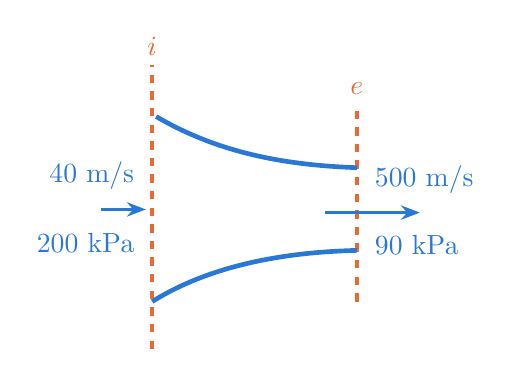
\begin{tikzpicture}[x=1cm, y=1cm,
    sec/.style={duRed, dashed, line width=1.26pt},
    wallc/.style={duBlue, line width=1.68pt},
    flow/.style={-{Stealth[length=2.4mm]}, duBlue, line width=1.26pt},
    val/.style={duBlue, font=\normalsize}]
  % inlet and exit sections
  \draw[sec] (0,-1.85) -- (0,1.75);
  \node[duRed, anchor=south] at (0,1.75) {$i$};
  \draw[sec] (2.6,-1.25) -- (2.6,1.25);
  \node[duRed, anchor=south] at (2.6,1.25) {$e$};
  % converging walls
  \draw[wallc] (0.05,1.1) .. controls (0.9,0.6) and (1.8,0.48) .. (2.6,0.45);
  \draw[wallc] (0.0,-1.25) .. controls (0.8,-0.75) and (1.8,-0.62) .. (2.6,-0.6);
  % inlet state
  \node[val, anchor=south east] at (-0.1,0.05) {$40~\mathrm{m/s}$};
  \draw[flow] (-0.65,-0.08) -- (-0.08,-0.08);
  \node[val, anchor=north east] at (-0.1,-0.25) {$200~\mathrm{kPa}$};
  % exit state
  \node[val, anchor=south west] at (2.7,0.0) {$500~\mathrm{m/s}$};
  \draw[flow] (2.2,-0.12) -- (3.4,-0.12);
  \node[val, anchor=north west] at (2.7,-0.28) {$90~\mathrm{kPa}$};
\end{tikzpicture}
\end{document}
